\documentclass[prb,showpacs,10pt,superscriptaddress]{revtex4-1}
%\documentclass[twocolumn,prb,showpacs,10pt]{article}
\usepackage{textcomp}
\usepackage{amsmath}
\usepackage{amssymb}
\usepackage{fontenc}
\usepackage{graphicx}
\usepackage{graphics}
\usepackage{subfig}
%\usepackage{float} \floatstyle{boxed} \restylefloat{figure}
\def\bra#1{\mathinner{\langle{#1}|}}
\def\ket#1{\mathinner{|{#1}\rangle}}
\def\braket#1{\mathinner{\langle{#1}\rangle}}
\usepackage{color}
\usepackage{multirow}
\usepackage{float} \restylefloat{figure}
\bibliographystyle{apsrev}
\usepackage[dvips]{hyperref}
\usepackage[justification=centering]{caption}
%\usepackage[utf8]{inputenc}
%\usepackage{authblk}
\usepackage{lipsum}
\makeatletter
\newcommand{\rmnum}[1]{\romannumeral #1}
\newcommand{\Rmnum}[1]{\expandafter\@slowromancap\romannumeral #1@}
\usepackage{amsmath,amsfonts}

%\date{\today}



\begin{document}

\title{Bridging Microscopic to Macroscopic Transport Through Functionalized Surfaces}
\author{Xin Zhao
\\Institute for Theoretical Physics, TU Wien, Wiedner Hauptstrasse 8-10, A-1040 Vienna, Austria}
%\affiliation{Institute for Theoretical Physics, TU Wien - Vienna University of Technology, Wiedner Hauptstrasse 8-10, A-1040 Vienna, Austria}
\begin{abstract}
In this proposal, I put emphasis on the functionalized surface where a single molecule is grafted on, within the crystalline/spacer/molecule interface, an interesting model of a classic Donor-spacer-Acceptor system is built, where Marcus theory can be applied to calculate the dynamics of the electrochemically driven electron transport process. 
\end{abstract}
\maketitle

\section{Introduction}
Thermoelectric materials and thermoelectric devices hold the promise for helping issues related to energy conversion and refrigeration~\cite{A review on thermoelectric renewable energy}. Compared to traditional refrigeration and heating devices, semiconductor based electronic components have the advantage of simplicity, and can be operated reliably at ambient temperatures and are highly scalable.

The challenges to enhance the figure of merit (ZT) for thermoelectric materials lies in the interplay between heat and charge, \textacutedbl phonon-glass electron-crystal \textgravedbl, which means low lattice thermal conductivity as a glass and high electrical conductivity as a crystal (Solid State Physics, Vol 34, 1st Edition). There are two ways to improve the thermoelectric properties: increasing the power factor ($\sigma S^2$) by optimizing the carrier concentration; reducing the lattice thermal conductivity by introducing scattering centers (defects).  

Heterojunctions \cite{thermoelectric in Molecular junction} are ideal in the sense that they provide efficient electron transport through frontier orbitals (HOMO or LUMO) and have a very low vibrational heat conductance due to the mismatch of vibrational spectra between electrodes (bulk metal) and discrete molecules \cite{Room temperature thermal conductance of alkanedithiol self-assembled monolayers}. Thermoelectric energy conversion efficiency can be achieved if charge transport occurs through a single energy level (reversible diffusive electron transport)\cite{Reversible Thermoelectric Nanomaterials}.
Molecular electronics is characterized by different transport mechanisms compared with conventional bulk crystalline conductors, which gives the new possibility to tune electronic couplings and design thermoelectric devices and sensors\cite{thermoelectric in Molecular junction,thermopower measurements in molecular junctions,Transition from strong to weak electronic coupling in a single-molecular junction}. To explore nanoscale electronics, a choice of the contacts for the molecular junction is critical.
Materials such as oxides, chalcogenides, semiconductors like SiGe, GaAs and recently monocrystalline SnSe \cite{two-step phase transition in SnSe} were found to possess high thermopower values. The efficiency of a thermoelectric material is measured by figure of merit (dimensionless),

\begin{equation}
 ZT = \dfrac{\sigma S^2}{K_{e} + K_{th}} T
\end{equation}
here $\sigma$ is the electric conductivity, $K_{e}$ and $K_{th}$ are the respective thermal conductivities due to electron and lattice phonon contributions, $S$ is the Seebeck coefficient.

\begin{figure}
%\begin{center}
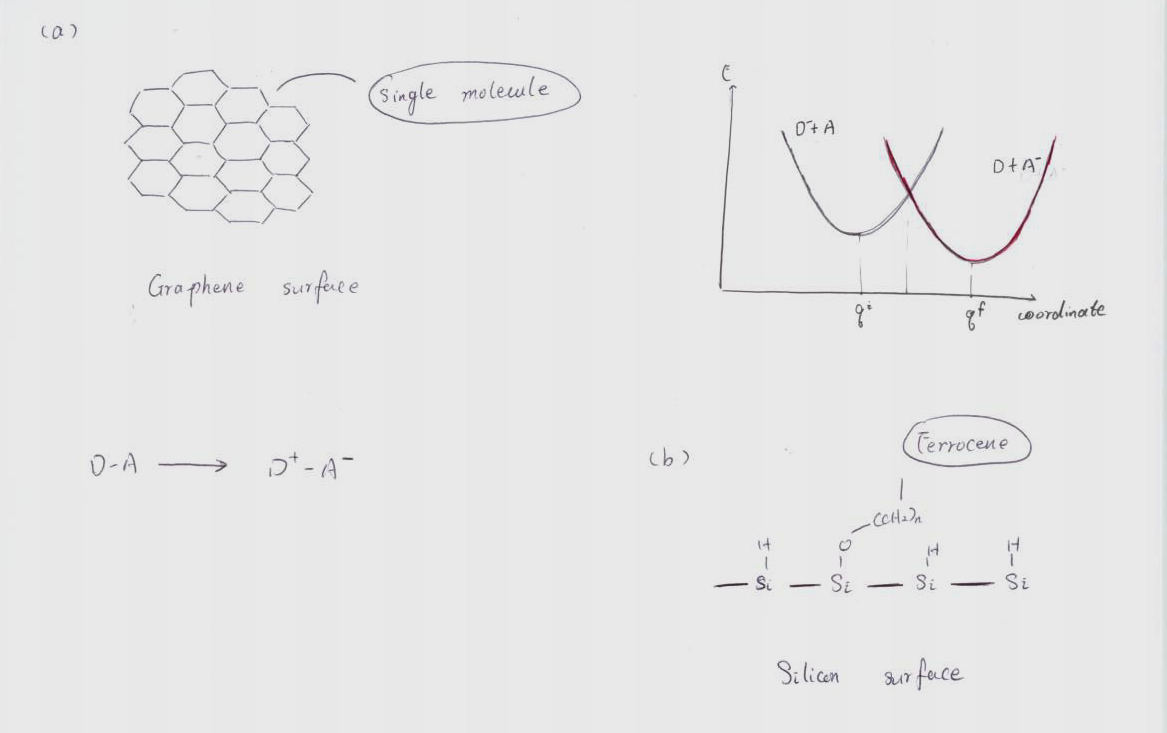
\includegraphics[width=1.\linewidth,angle=0]{interface_scheme.png}
\caption{\small Models for crystalline/spacer/molecule interface representative of donor-spacer-acceptor within Marcus framework.}
%\end{center}
\end{figure}


\section{Models}
The idea to bring together single molecules and polycrystalline via surface functionalization is aimed at bridging the knowledge I have acquired and the research direction of interest in your group, with an emphasis on exploring how it can be realized utilizing widely used codes and theories. Meanwhile it's intriguing to develop methods when necessary. The models are shown in Figure 1, where (a) is the graphene polycrystalline as electrodes, where intrinsic topological defects of grain boundaries are expected to alter the electronic transport. Yazyev \textit{et al.} found a large on/off ratio (above 1,000) for a model field-effect transistor based on grain boundaries \cite{Electronic transport in polycrystalline graphene}. 
Another type of interface (b) is silicon(111)/organic-spacer/Ferrocene \cite{Ferrocene molecular architectures grafted on Si,XPS and electrochemical studies of ferrocene derivatives anchored on Si,Measurements of Electron-Transfer Rates of Charge-Storage}, where electron transfer rates at the interface are calculated by a constrained density functional theory method.    

%\par
\section{Break Junction Technique}
There are two ways of measuring the thermopower in molecular junctions, namely voltage measurements techniques \cite{thermoelectric in Molecular junction} and thermoelectric current measurements techniques \cite{Simultaneous Determination of Conductance and Thermopower of Single Molecule Junctions, Engineering the Thermopower of C60 Molecular Junctions}, where for the latter method the electronic conductance and thermopower can be measured in the same junction simultaneously.
Expressions for conductance and thermopower in molecular junction under the low temperature limit and not too close to transmission resonances,
\begin{equation}
 G= \dfrac{2e^2}{h}\mathcal{T}(E_{f})
\end{equation}
\begin{equation}
 S(T)= -\dfrac{\pi^2}{3}\dfrac{k_{B}^2T}{e}\dfrac{1}{\mathcal{T}(E)}\dfrac{d\mathcal{T}(E)}{dE}\Bigg |_{E_{f}}
 \label{thermopower}
\end{equation}
where $\mathcal{T}(E)$ is the transmission probability, and $E_{f}$ is the Fermi level. From the eq. ~\ref{thermopower} it's obvious that when transmission function $\mathcal{T}(E)$ changes rapidly around the Fermi level, a large thermopower can be achieved. Quantum interference (QI) effects which induce a steep gradient in the transmission function therefore can be linked to thermoelectric efficiency as an important factor \cite{controlling the transmission line shape and potentional thermoelectric applications,Giant Thermoelectric Effect from Transmission Supernodes}.

\section{Theories}
In order to bridge the charge transport through single molecules and polycrystalline materials, three mechanisms are involved: Landaur formular for coherently (ballistic) transport in the nanoscale molecular junctions, Boltzmann equation for diffusive transport and phonon drag in crystalline, Marcus theory framework for calculating the electron hopping rates at the interfaces. 
\subsection{Marcus Theory}
The three key parameters for calculating the charge transfer dynamics within Marcus framework are i)the reorganization energy ($\lambda$); ii)the driving force (the energy difference between the reagents and products $\Delta E^{react}$); iii)the transfer integral ($V_{DA}$)\cite{DFT calculations for tranfer intergral}. 
In the case of an electron transfer occurring at the interface,
\begin{equation}
 k_{ET} = \dfrac{2\pi}{\hbar}V_{DA}^2 \dfrac{1}{\sqrt{4\pi\lambda k_{B}T}}exp(-\dfrac{\Delta E_{f}^{act}}{k_{B}T})
\end{equation}
where $\lambda = \lambda_{in} + \lambda_{out}$ is the sum of inner and outer reorganization energies. $\Delta E_{f}^{act}$ can be calculated from $\lambda$ and $\Delta E^{react}$. $V_{DA}$ is the transfer integral between the donor and acceptor states.

\subsection{Boltzmann Equation}
%\begin{align}
\begin{equation}
\frac{\partial f}{\partial t} + \dot{\textbf{r}}\frac{\partial f}{\partial \textbf{r}} + \dot{\textbf{p}}\frac{\partial f}{\partial \textbf{p}} = - \int\int\int d^3 p_{1}d^3p^{\prime}d^3p_{1}^{\prime} \sigma(\textbf{p},\textbf{p}_{1} 
\longrightarrow \textbf{p}^{\prime},\textbf{p}_{1}^{\prime}) \dfrac{1}{m} \mid \textbf{p}-\textbf{p}_{1} \mid (ff_{1}-f^{\prime}f_{1}^{\prime})
\end{equation}


%\end{align}
where $f$ is the one-particle distribution function $f=f(\textbf{r},\textbf{p},t)$, $f_1=f(\textbf{r},\textbf{p}_{1},t)$,  $f^{\prime}=f(\textbf{r},\textbf{p}^{\prime},t)$, $f_{1}^{\prime}=f(\textbf{r},\textbf{p}_{1}^{\prime},t)$.
\

\subsection{Landauer-B\"{u}ttiker Formalism and Green's Function}
For ballistic transport, the single-channel current from left to right is,
\begin{equation}
I= \dfrac{2q}{\hbar} \int_{-\infty}^{\infty} dE \mathcal{T}(E) [f_{L}(\varepsilon) - f_{R}(\varepsilon)]
\end{equation}
where $f_{L,R}(E)$ is the Fermi Dirac distribution for the left and right electrodes.
The Green's Function of the scattering region in the molecular junctions defines the transmission function $\mathcal{T}(E)$, which is calculated as,
\begin{equation}
G_{C} = [E\textbf{I} - \textbf{H} - \Sigma_{L} - \Sigma_{R}]^{-1}
\end{equation}
where self-energy matrices $\Sigma_{L/R}$ are introduced for describing the broadening due to the couplings to the source and drain, $\textbf{I}$ is identity matrix.
\begin{equation}
\mathcal{T}(E) = \textbf{Trace}[\Gamma_{L} G_{C}(E) \Gamma_{R} G_{C}^\dagger(E)]
\end{equation}
$\Gamma_{L/R}$ are the coupling matrices of left and right electrodes, respectively. 

In short summary, the combination of single molecules and polycrystalline as single molecular junctions might improve the thermoelectric energy conversion efficiency of heterojunctions, and the suggested techniques would allow to assess this hypothesis. There are several strategies for tuning the thermopower, for instance, introducing chemical moieties in the molecule, varying the length or chemical bonding at the metal-molecular interface, or the number of the molecules trapped in the junctions.   
When dealing with such interfaces charge transfer, the impact of interface dipole needs to be considered, a topic on which I already did some studies in collaboration with an experimental group. (M. Lemmer, X. Zhao, R. Stadler and T. Albrecht, in preparation (2018))
%\newpage


\bibliographystyle{apsrev}

\bibliographystyle{apsrev}

\begin{thebibliography}{}
\bibitem{A review on thermoelectric renewable energy}H, Alam, S. Ramakrishna, \textit{Nano Energy}, \textbf{2}, 190-212(2013).
\bibitem{thermoelectric in Molecular junction}P. Reddy, S.-Y. Jang, R.A. Segalman, A. Majumdar, \textit{Science}, \textbf{315}, 1568-1571(2007).
\bibitem{thermopower measurements in molecular junctions}L. Rinc\'{o}n-Garc\'{\i}a, C. Evangeli, G, Rubio-Bolling and N. Agra\"{\i}t,  \textit{Chem. Soc. Rev.}, \textbf{45}, 4285-4306(2016).
\bibitem{Transition from strong to weak electronic coupling in a single-molecular junction}R. Frisenda and H. S. J. van der Zant,  \textit{Phys. Rev. Lett.}, \textbf{117}, 126804(2016).
\bibitem{Room temperature thermal conductance of alkanedithiol self-assembled monolayers}R.Y. Wang, R.A. Segalman, A. Majumdar,  \textit{Appl. Phys. Lett.}, \textbf{89}, 173113(2006).
\bibitem{Reversible Thermoelectric Nanomaterials}T.E. Humphrey, H. Linke, \textit{Phys. Rev. Lett.}, \textbf{94}, 096601(2005).  
\bibitem{two-step phase transition in SnSe}A. Dewandre, O. Hellman, S. Bhattacharya, A.H. Romero, G.K.H, Madsen and M.J Verstraete, \textit{Phys. Rev. Lett.}, \textbf{117}, 276601(2016).
\bibitem{Electronic transport in polycrystalline graphene}O.V. Yazyev and S.G. Louie, \textit{Nat. Mater.}, \textbf{9}, 806–809(2010).
\bibitem{Ferrocene molecular architectures grafted on Si}C. Fontanesi, M. Innocenti,D. Vanossi, and E. Da Como, \textit{Materials}, \textbf{10}, 1109(2017).
\bibitem{XPS and electrochemical studies of ferrocene derivatives anchored on Si}
\bibitem{Measurements of Electron-Transfer Rates of Charge-Storage}K.M. Roth, A.A. Yasseri, Z. Liu, R.B. Dabke,
V. Malinovskii, K.-H. Schweikart, L. Yu, H. Tiznado,F. Zaera, J.S. Lindsey, W.G. Kuhr and D.F. Bocian, \textit{J. Am. Chem. Soc.}, \textbf{125}, 505–517(2003).
\bibitem{Simultaneous Determination of Conductance and Thermopower of Single Molecule Junctions}J.R. Widawsky, P. Darancet, J.B. Neaton and L. Venkataraman, \textit{Nano Lett.}, \textbf{12}, 354-358(2012).
\bibitem{Engineering the Thermopower of C60 Molecular Junctions}C. Evangeli, K. Gillemot, E. Leary, M.T. Gonz\'{a}lez, G. Rubio-Bollonger, C.J Lambert and N. Agra\"{\i}t, \textit{Nano Lett.}, \textbf{13}, 2141-2145(2013).
\bibitem{controlling the transmission line shape and potentional thermoelectric applications}R. Stadler and T. Markussen, \textit{J. Chem. Phys.}, \textbf{135}, 154109(2011).
\bibitem{Giant Thermoelectric Effect from Transmission Supernodes}J.P. Bergfield, M.A. Solis and C.A. Stafford, \textit{ACS Nano}, \textbf{4}, 5314(2010).
\bibitem{DFT calculations for tranfer intergral}G. Kastlunger and R. Stadler, \textit{Phys. Rev.} B, \textbf{89}, 115412(2014).

\end{thebibliography}
\end{document}

